\subsection{POC 1: Commenting Module for Events in Indico}

The first \gls{poc} is supposed to enrich the Indico system with some sort of Solid-based content. With the product owner and chief developer of Indico, the CERN-Solid project manager, and a Solid developer it was decided a commenting module for Indico events is an adequate solution to include data from an external storage entity namely a data pod. The ability to allow users of Indico to leave a comment on an event, which then lives in a data pod completely controlled by the author of the comment was concluded to be an attractive feature for Indico.

\subsubsection{Architectural Analysis and Synthesis}\mbox{}\\

In this section, the architectural analysis will be looked into. The scope of the system and its attributes will be defined based on the system description and the quality attributes from the analysis of stakeholder needs.

\paragraph{System Description}\mbox{}\\

The system aims at enabling commenting in web applications with decentralized storage on data pods. The system in the context of Indico intends to allow Indico users with a data pod to comment on specific Indico events.

\paragraph{Features}\mbox{}\\

The core functionality of the module consists of the following three features: 

\vspace{-12mm}
\begin{enumerate}
    \item A user with a Solid account can authenticate with their Solid \gls{idp}
    \item A user can compose a text which is stored on their data pod
    \item A user can see other users’ comments
\end{enumerate}
\vspace{-10mm}

These features allow the development of a module giving users the ability to authenticate themselves using their WebID, storing the created data in form of comments in their own data pod, and also see decentralized stored data from other users.

\paragraph{Type of Users}\mbox{}\\

There are two types of users in the system. The first group of users is the active authors of comments or observers of such. These will interact with the module by logging in to their data pod and compose comments. The other subset of users is the administrators of the application (Indico). This type of user is interested in keeping the tone of comments to the community guidelines and not allow any misuse.

\paragraph{Context Diagram}\mbox{}\\

Other types of involved parties are the ones maintaining or developing the system and application. These are shown in the context diagram \ref{fig:poc-comment-context_diagram}.

\begin{figure}[H]
    \centering
    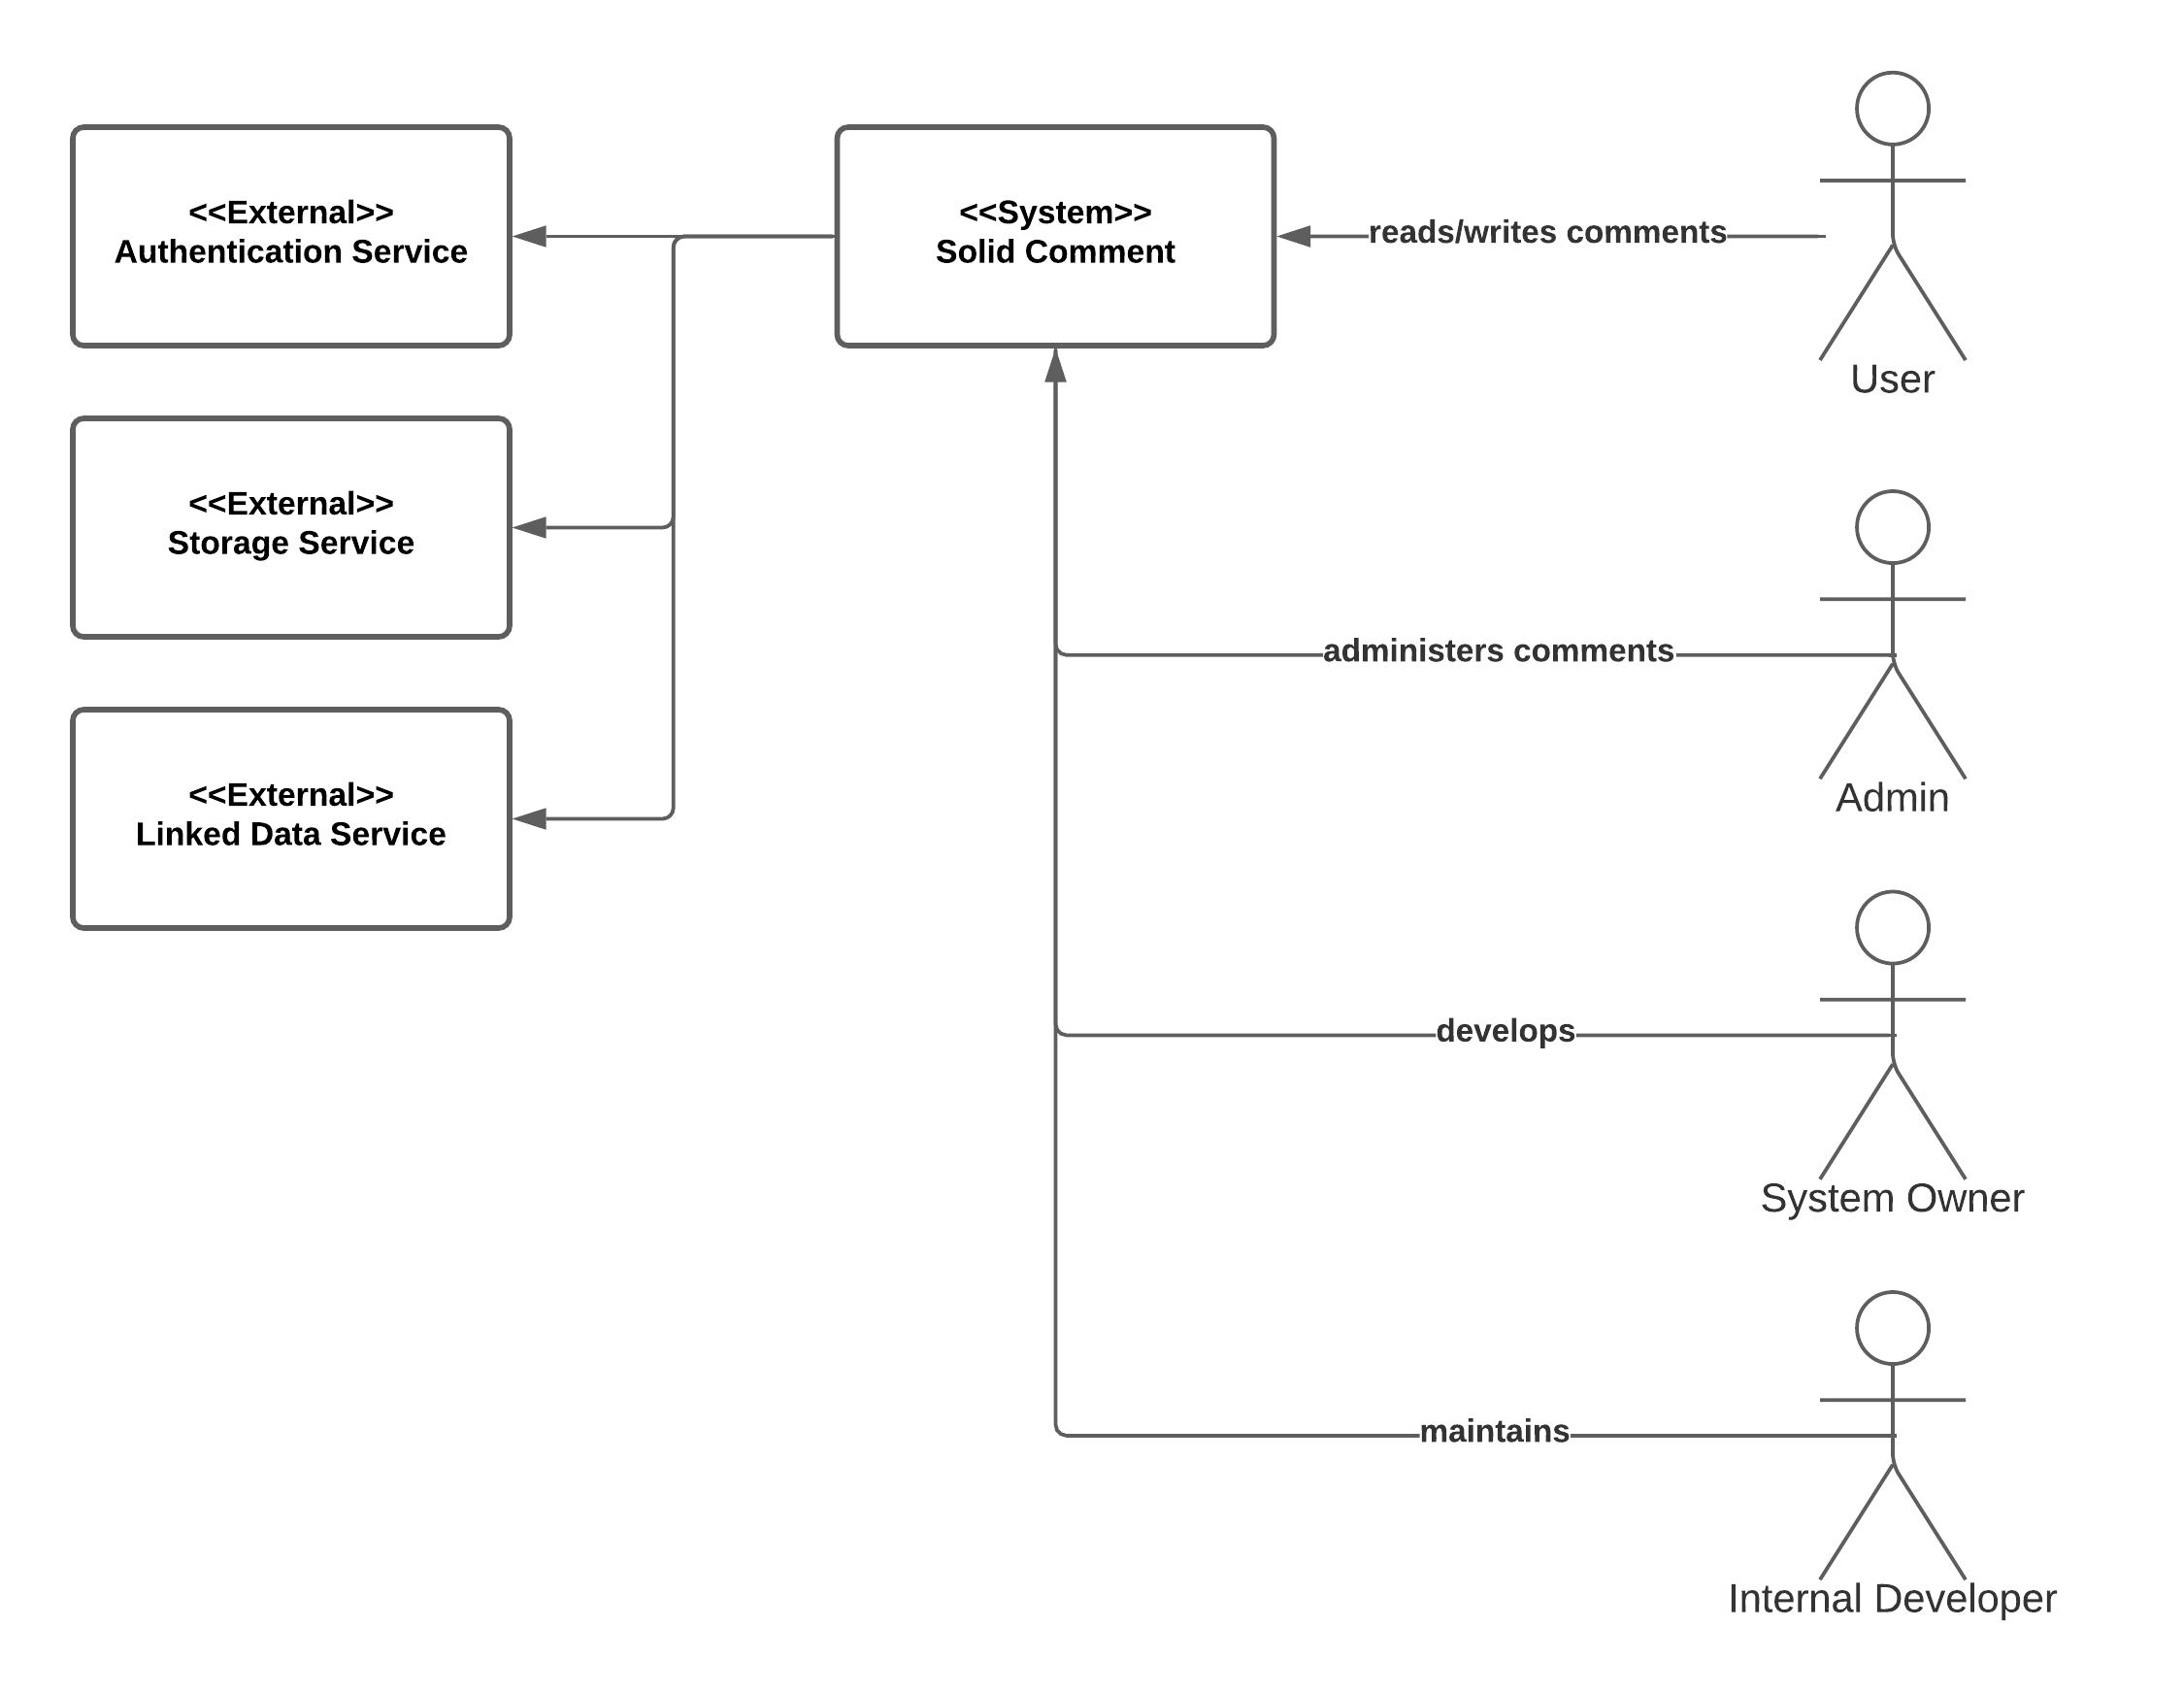
\includegraphics[width=0.8\textwidth]{prototype/graphs/poc-comment-context_diagram.png}
    \caption{Context diagram showing users and external services of system.}
    \label{fig:poc-comment-context_diagram}
\end{figure}

\paragraph{Sequence Diagram}\mbox{}\\

A sequence diagram brings a suitable overview for any software architecture, but especially useful for decentralized systems or those containing several separate services. It gives a clear understanding of each service’s tasks and their relationship when passing messages around in the overall system.

\begin{figure}[H]
    \centering
    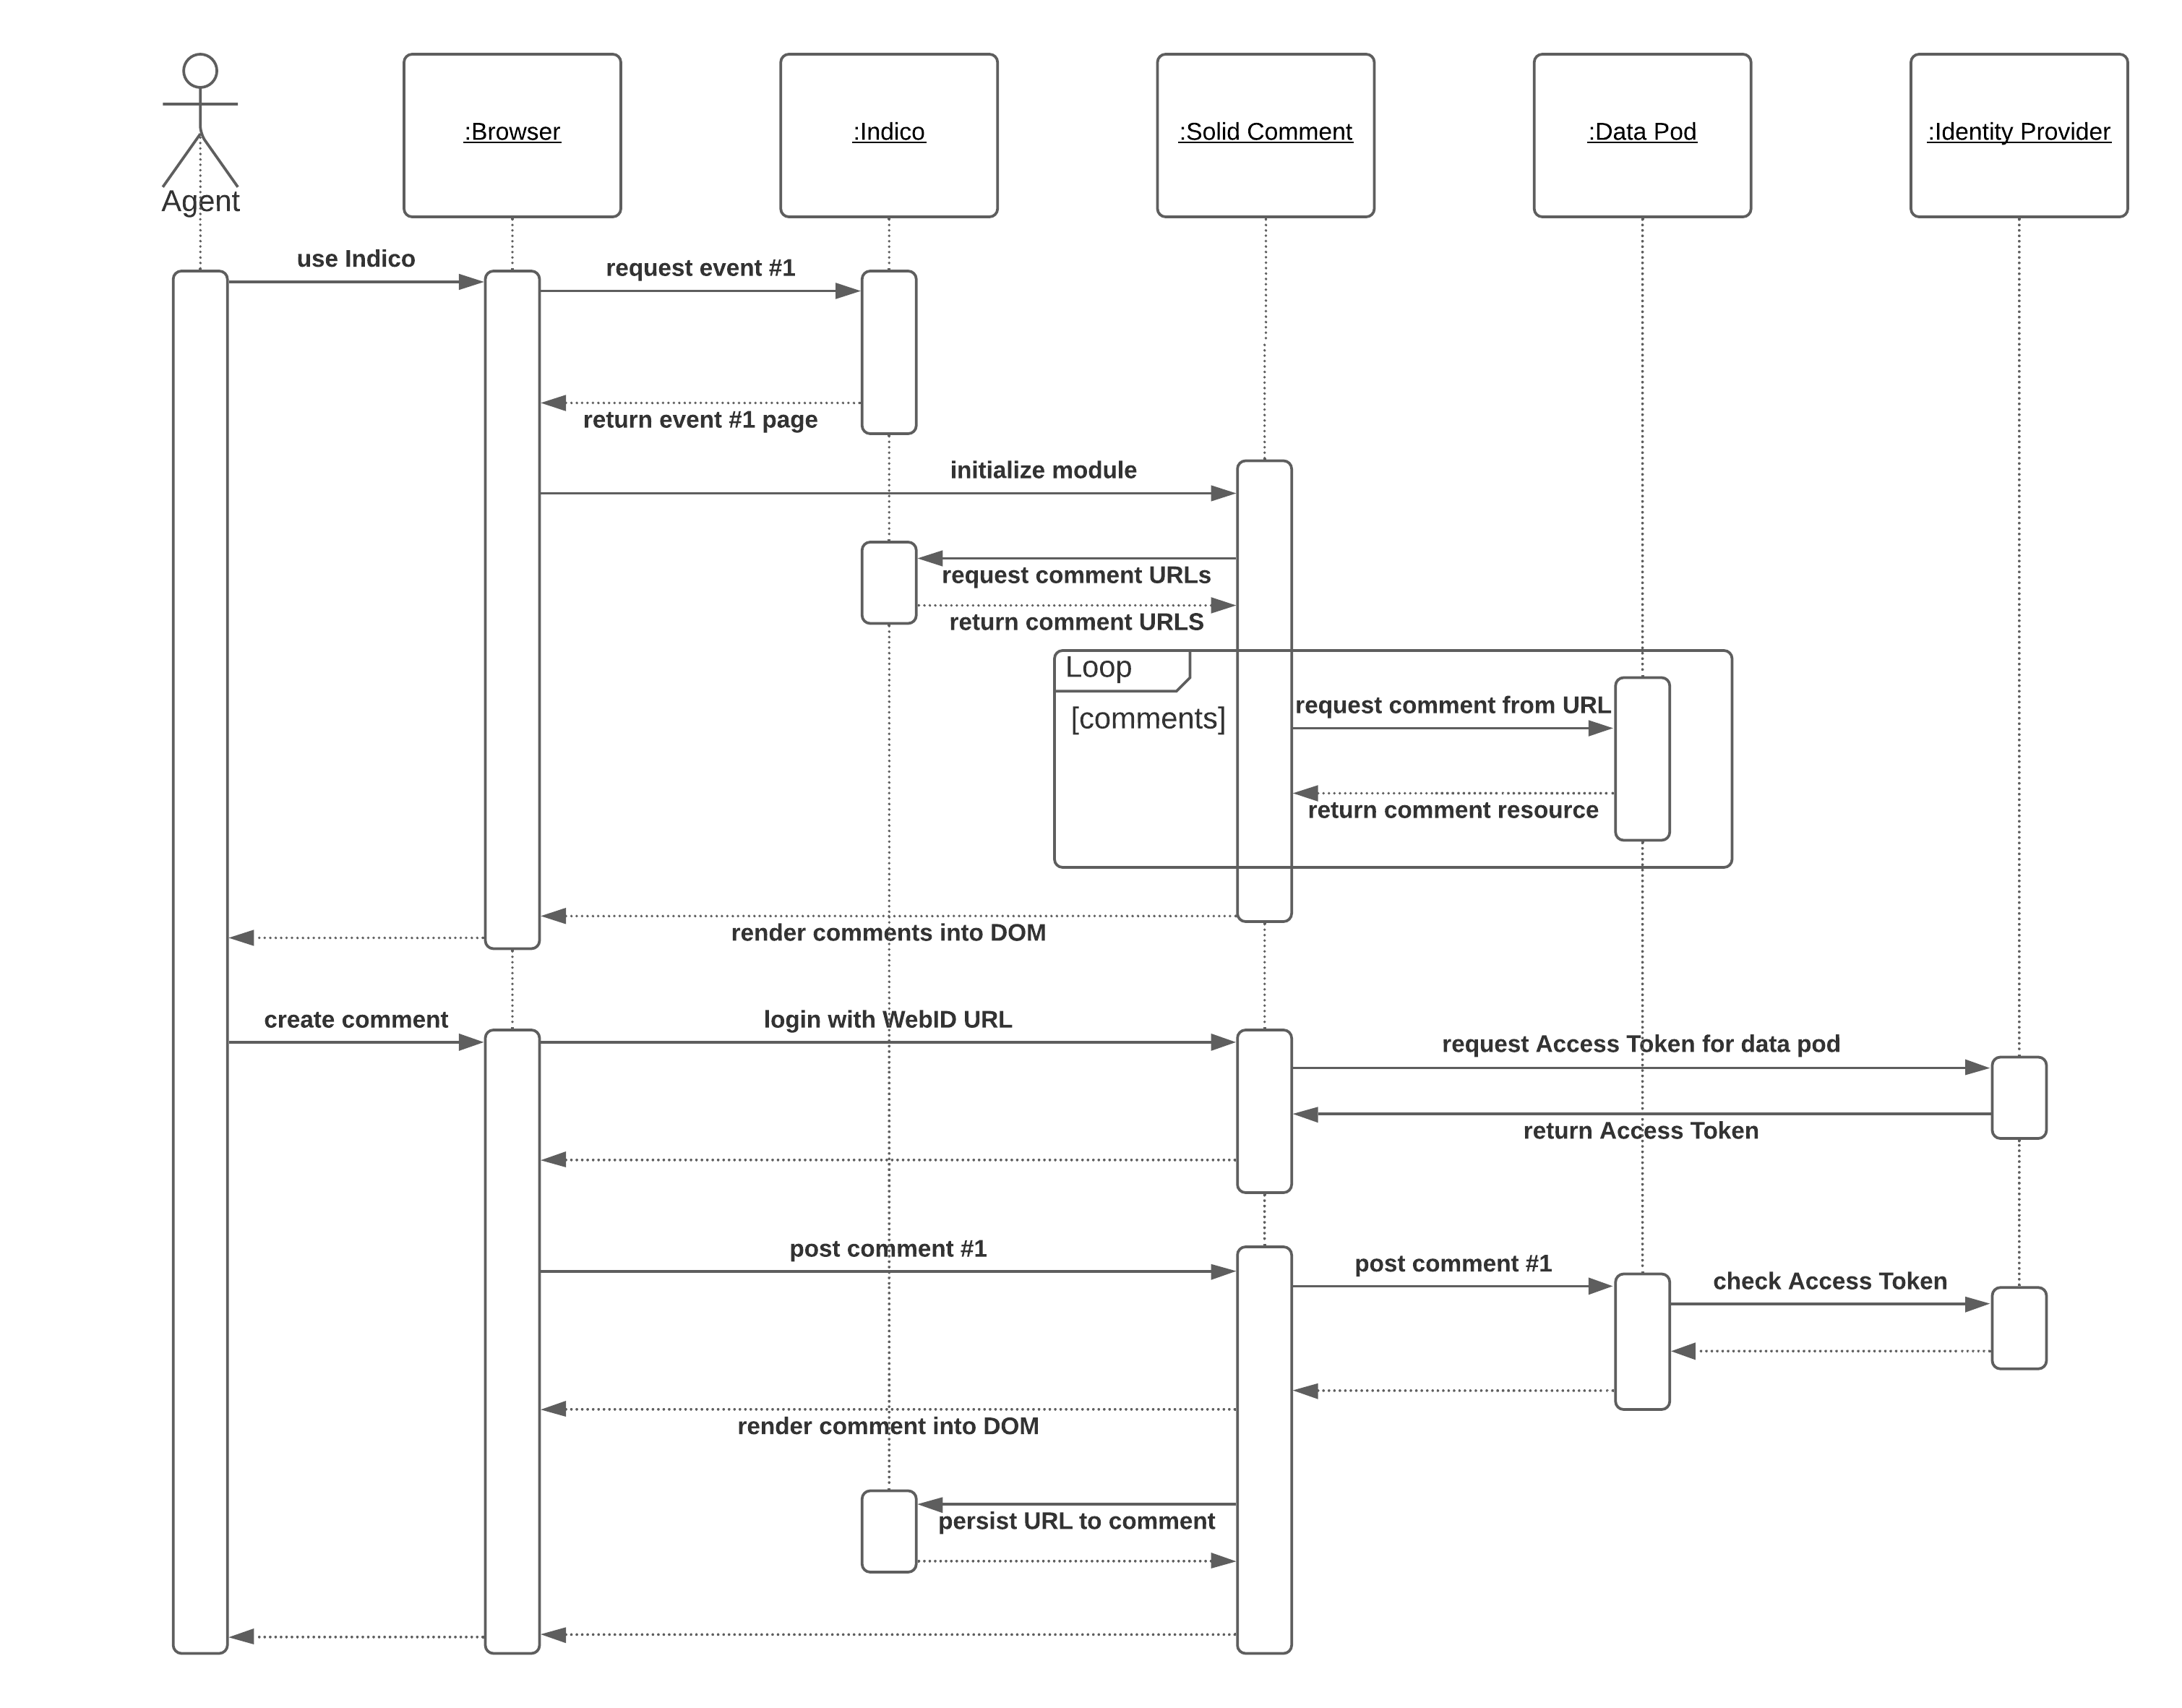
\includegraphics[width=\textwidth]{prototype/graphs/poc-comment-sequence_diagram.png}
    \caption{Sequence diagram showing the sequential process through posting a comment.}
    \label{fig:poc-comment-sequence_diagram}
\end{figure}

\paragraph{Stakeholders}\mbox{}\\

This section covers the various stakeholders in relation to the system. This both includes active users, but also various external and internal stakeholders who are impacted by the system or have an important say in the development process.

The \textbf{product owner} is responsible for the product, in this case, Indico. Usually, they are the ones planning repeated fixed time-boxes in which new features are developed or the existing software is maintained. They are constantly evaluating the state of the software and try to satisfy other stakeholders such as investors or the system users themselves. The main concerns of the product owner are to stay innovative while no compromising the quality of the existing software.

The \textbf{internal developer} is responsible for executing the decision made by, or together with, the product owner. The developer is also maintaining the software and is the one working with it on a daily basis and can, therefore, make assumptions about the evolution of the software. Their concerns lie in the maintainability of the software through its evolutionary cycle, as well as onboarding new developers.

\paragraph{Drivers}\mbox{}\\

The architectural driver or quality attributes can be specified using “-illities”

\begin{enumerate}
    \item Security
    \item Performance
    \item Usability
\end{enumerate}

\subsubsection{Screen Design}\mbox{}\\

For various meetings and presentations, a visual representation of the to-be-developed module helps to guide the audience through the process. For the comment module, a user interface was designed in graphical software to ease the explanation of the goals for this module. The existing Indico design was adopted to blend into the system.

\begin{figure}
    \centering
    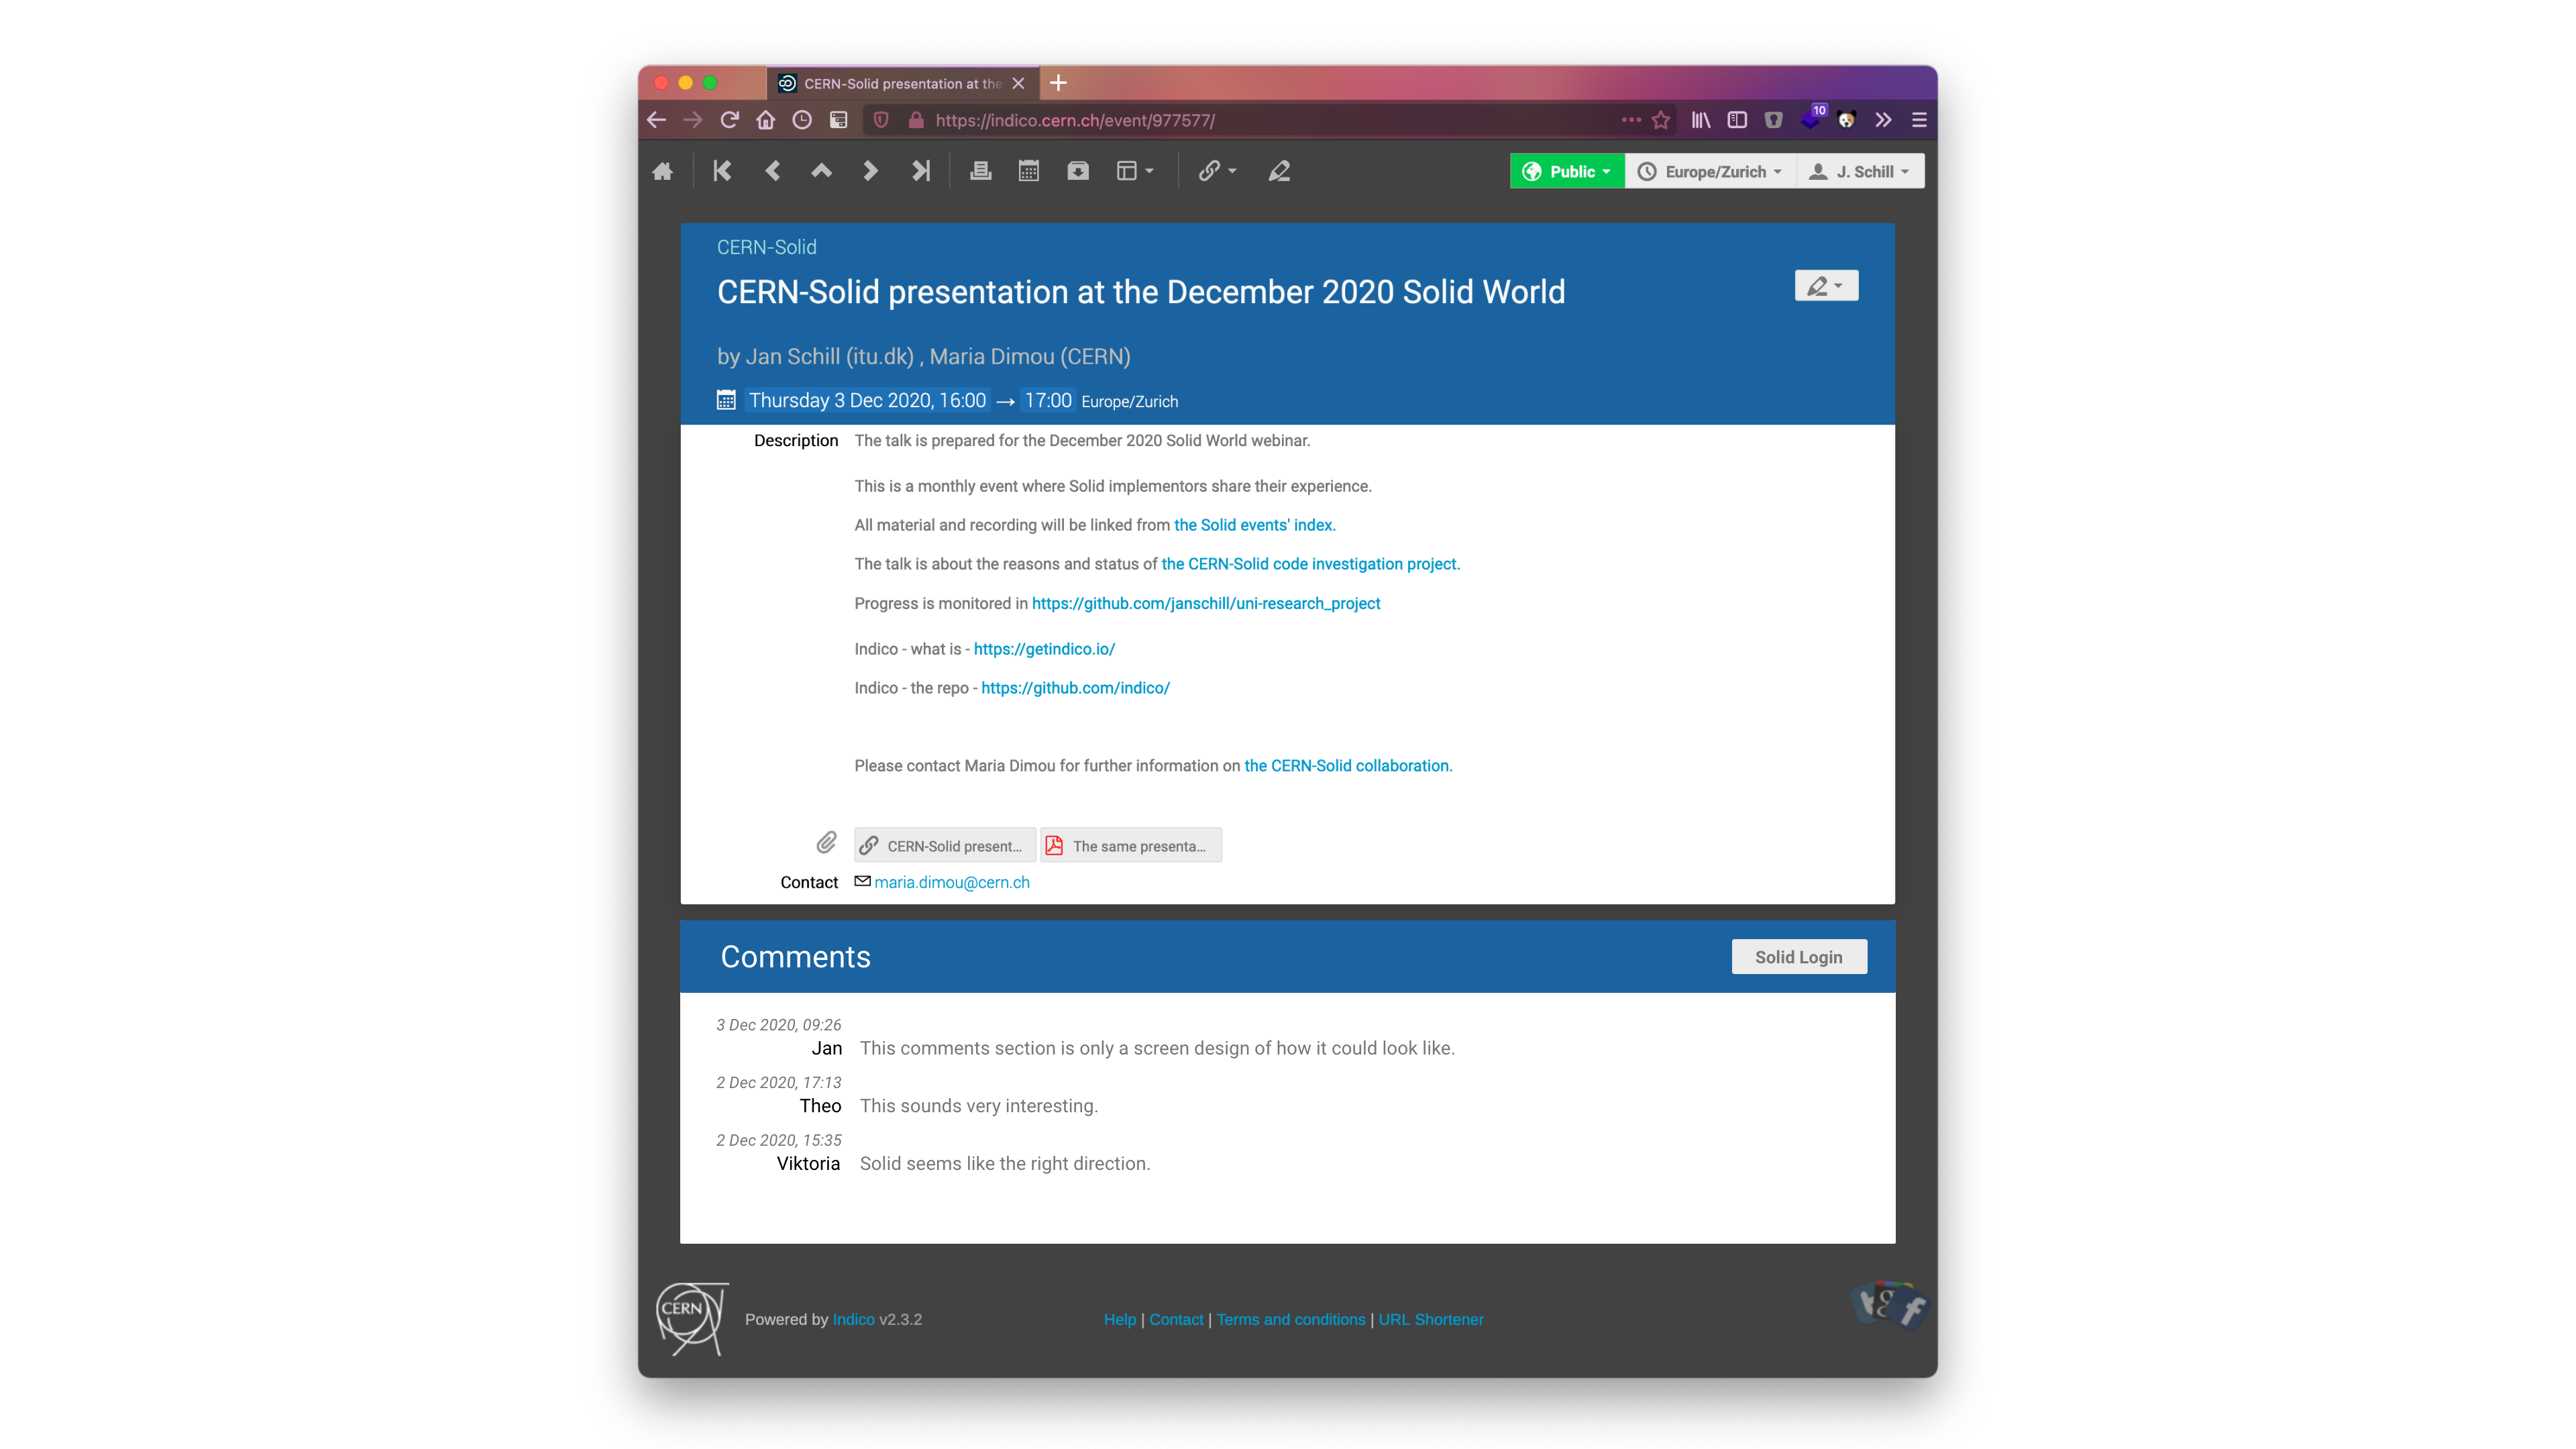
\includegraphics[width=1\textwidth]{prototype/screen_design/indico-comments-screen_design.png}
    \caption{User interface showing the comment module.}
    \label{fig:indico-comments-screen_design}
\end{figure}

\subsubsection{Design}\label{subsubsection:design}\mbox{}\\

For the implementation of this module, several design decisions had to be made. From the fundamental choice of the module running on the client device or be computed on the server and then propagated to the client afterward or even with a microservice proxying all traffic to enable Solid without changing Indico.
Other design challenges were around how to protect the resources holding the comment information. These resources reside on the external data pod and need to be fetched from the application and read by other agents. Can \glspl{acl} be configured to allow the specific use-case and other questions to come up and had to be considered?

\paragraph{Client- Versus Server-Side Versus Microservice}\mbox{}\\

When an agent browses to a running instance of Indico most of the functionality is being prepared on the server hosting Indico. It retrieves the specific request, builds the \gls{html}, and sends it to the user. For Indico most of the functionality is built with Python and the web framework Flask. Sometimes functionality needs to be closer to the user, an example is a dynamic rendering of \gls{dom} elements. This is useful when new data needs to be shown right away without getting the blank white screen on a page reload.
Indico does send \gls{js}, which is used for client-side features, but it focuses on keeping most of its features on the server.

To make the right decision if the module should be primarily developed for the client- or server-side or even as a microservice, a list of requirements to the module had to be defined. With the defined requirements in place, it had to be figured out how much functionality can be extracted from existing libraries and how much needed to be implemented with the new module. Implementing existing functionality for a new programming language would defeat the \gls{poc}’s purpose of showing how an existing software could work with the Solid principles.

The rudimentary set of features to enable commenting for users in Indico while saving the data in a data pod includes: 

\begin{enumerate}
    \item Authentication with a Solid \gls{idp}
    \item (Authenticated) Requests to a data pod
    \item Parsing of structured data (Linked Data)
\end{enumerate}

\paragraph{Client Approach}\mbox{}\\

The module runs in the browser and is therefore written in \gls{js}. A programming language which compiles to \gls{js}, such as \gls{ts}, is also possible. This means Indico remains mostly untouched but would have to serve the needed \gls{js} to the client on traffic to an event endpoint where the comment module is integrated.

\begin{table}[h!]
    \centering
    \begin{tabular}{| l | l |} 
     \hline
     Problem & Solution \\
     \hline
      Language & \gls{js} or \gls{ts}  \\
      Framework & Native \gls{js}  \\
      Client & solid-client-js \cite{solid-client-js}  \\
      Authentication & solid-client-authn-browser \cite{solid-client-authn-browser} \\
      RDF & solid-common-vocab-js \cite{solid-common-vocab-js}, rdflib.js \cite{rdflib.js}  \\
     \hline
    \end{tabular}
    \vspace{0.75cm}
    \caption{Existing solutions to problems for a client approach.}
    \label{table:1}
\end{table}

The communication flow with the data pod and the module would happen primarily from the browser.

\begin{figure}[H]
    \centering
    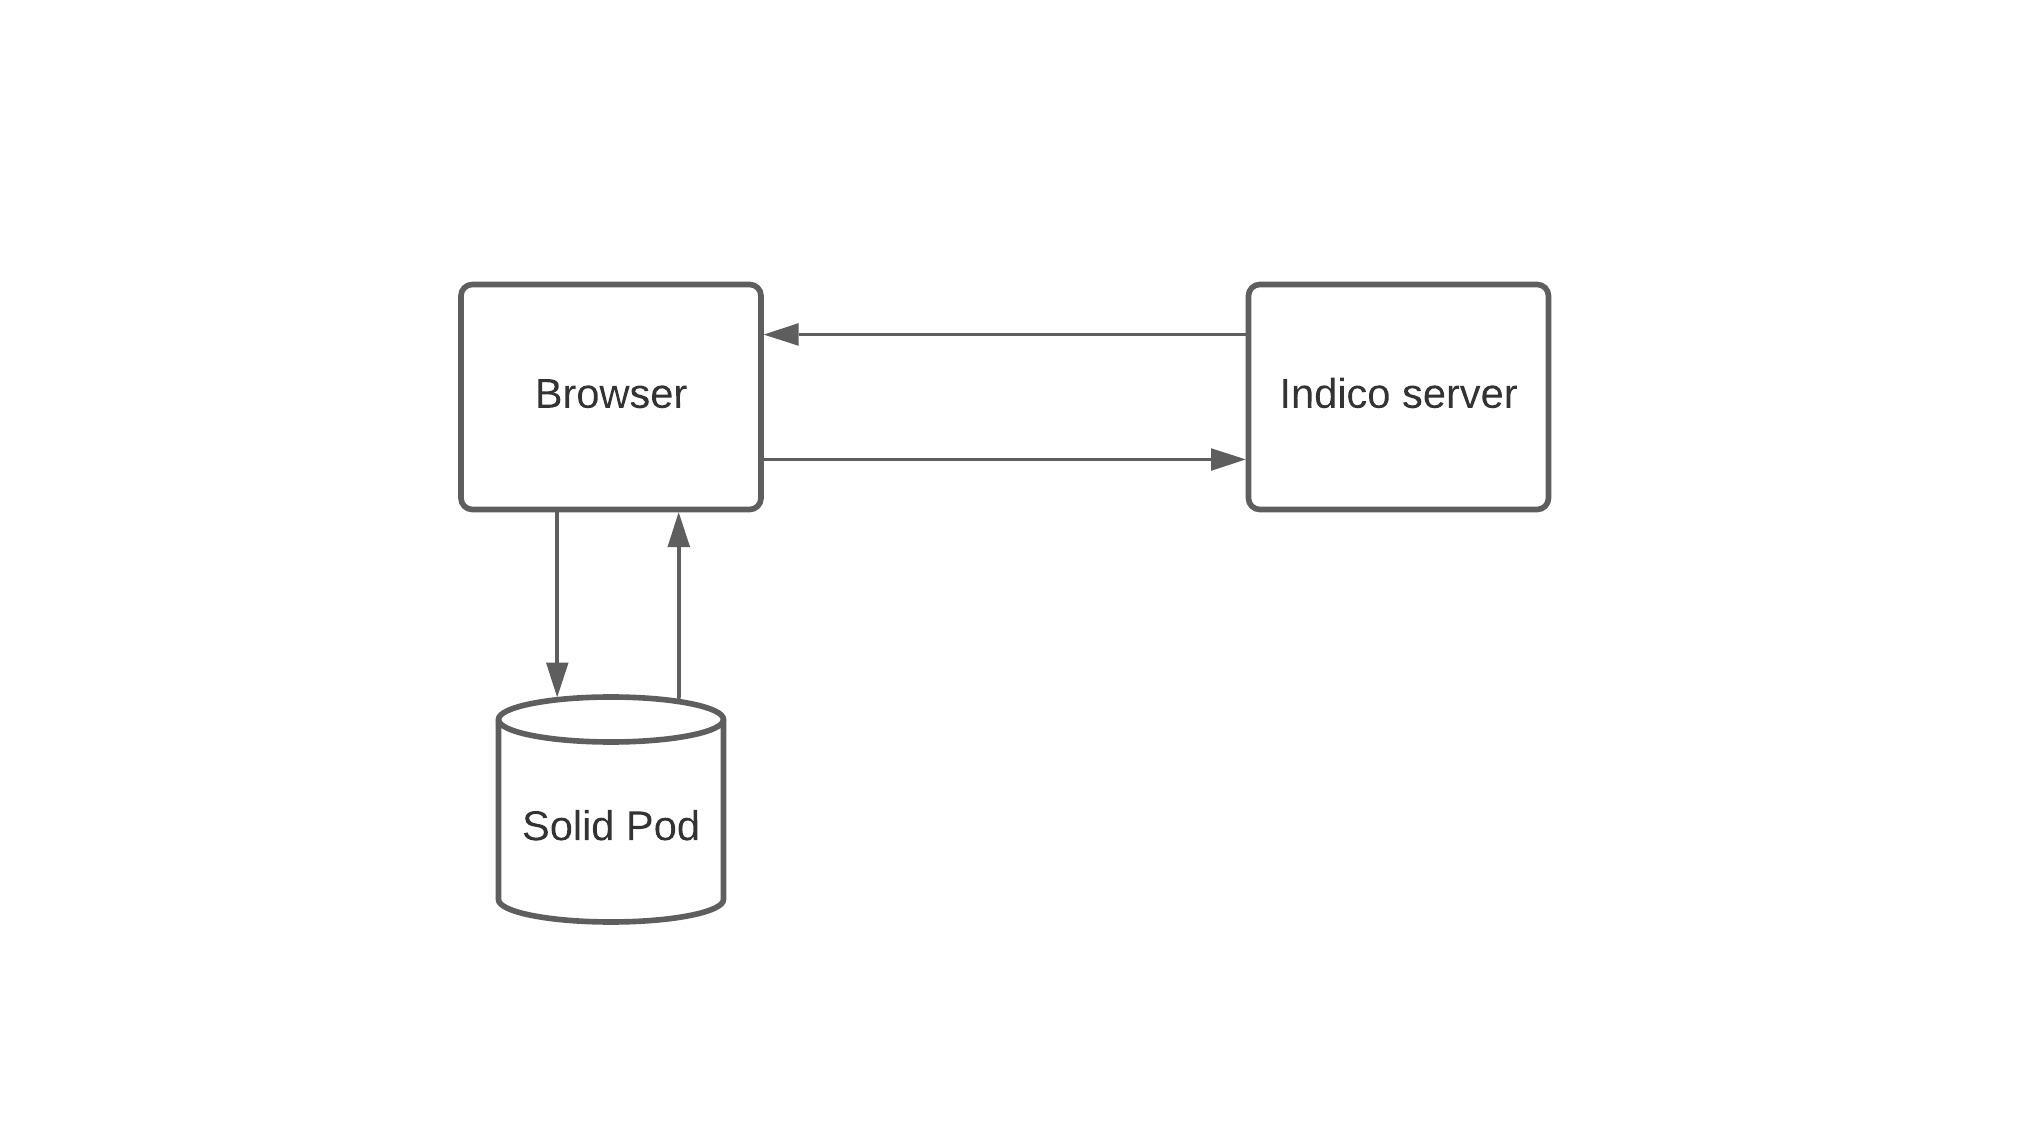
\includegraphics[width=0.8\textwidth]{prototype/graphs/poc-infrastructure-frontend.jpeg}
    \caption{Communication flow for a module developed on the client.}
    \label{fig:poc-infrastructure-frontend}
\end{figure}

\paragraph{Microservice Approach}\mbox{}\\

The microservice approach would allow developing the needed Solid logic on a separate service, which proxies all Solid related traffic through it and enables the Solid functionality. Most of the libraries from the client implementation can be used as well, as both developments would be written in \gls{js}. Only the authentication flow would work a bit differently.

\begin{table}[h!]
    \centering
    \begin{tabular}{| l | l |} 
    \hline
     Problem & Solution \\
     \hline
      Language & \gls{js} or \gls{ts}  \\
      Framework & Node.js  \\
      Client & solid-client-js \cite{solid-client-js}  \\
      Authentication & solid-client-authn-node \cite{solid-client-authn-node} \\
      RDF & solid-common-vocab-js \cite{solid-common-vocab-js}, rdflib.js \cite{rdflib.js}  \\
    \hline
    \end{tabular}
    \vspace{0.75cm}
    \caption{Existing solutions to problems for a microservice approach.}
    \label{table:2}
\end{table}

The microservice module would handle take all requests aimed at the data pod and make it compliant with the Solid server. It would provide the client with the proper \gls{solidoidc} flow to attach the access token to all authenticated requests.

\begin{figure}[H]
    \centering
    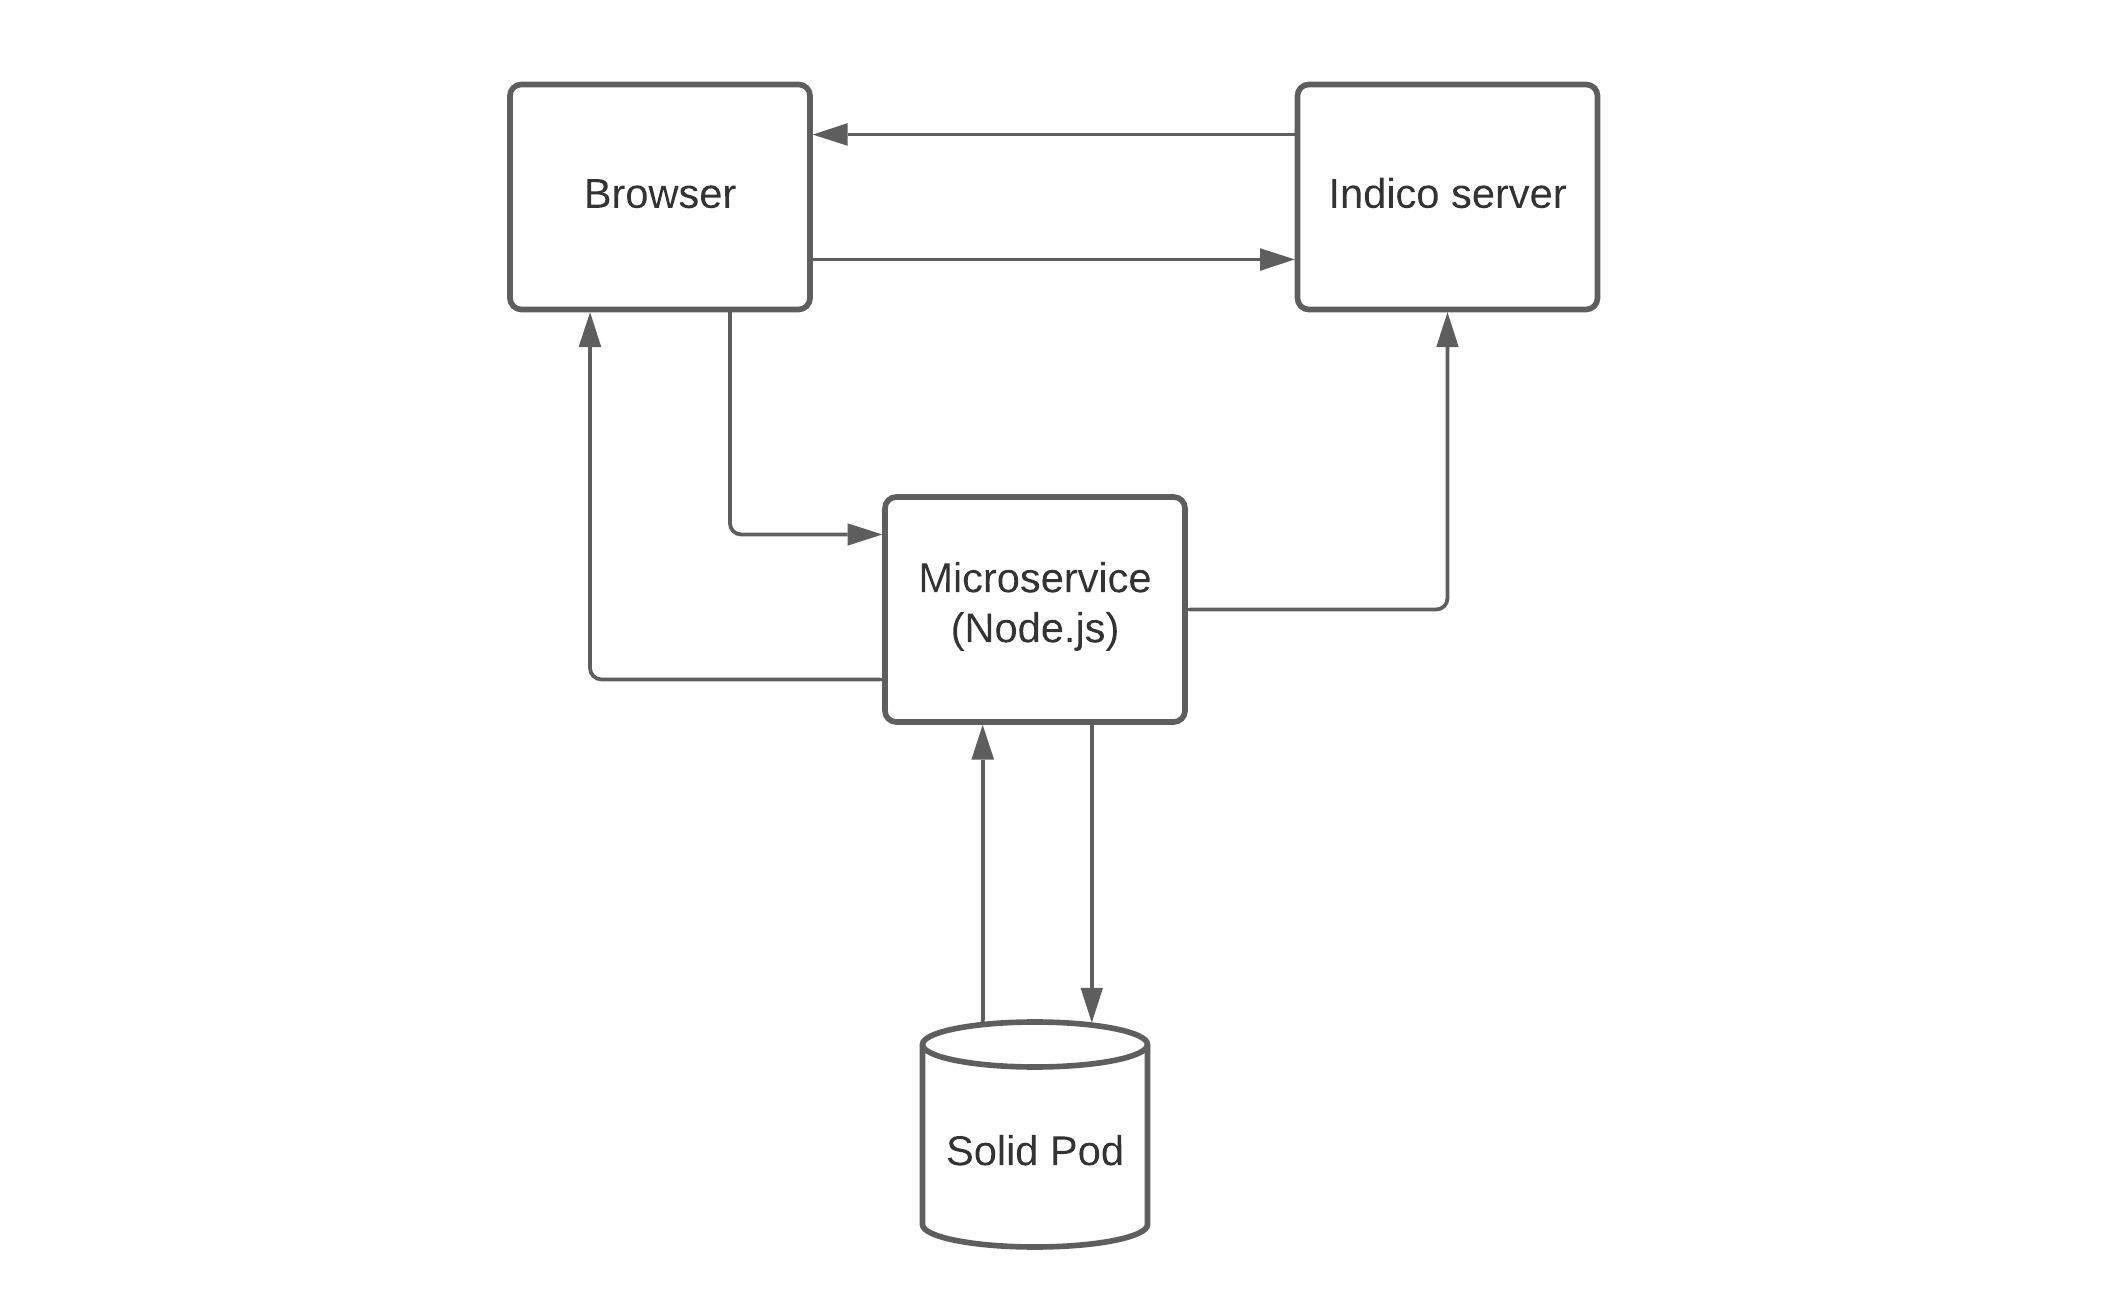
\includegraphics[width=0.8\textwidth]{prototype/graphs/poc-infrastructure-microservice.jpeg}
    \caption{Communication flow for a module developed as a microservice.}
    \label{fig:poc-infrastructure-microservice}
\end{figure}

\paragraph{Server Approach}\mbox{}\\

The goal of the server approach would be just like with the microservice approach to decouple the logic needed to work with Solid from the client and have it run on a server instance. The attractiveness for the server approach would be it could be fully integrated within Indico and be part of its Python codebase. The major drawbacks are no direct Solid libraries written in Python exist to allow a seamless integration into the ecosystem.

\begin{table}[!ht]
    \centering
    \begin{tabular}{| l | l |} 
    \hline
     Problem & Solution \\
     \hline
      Language & Python  \\
      Framework & Flask  \\
      Client & -  \\
      Authentication & pyoidc \cite{pyoidc} missing DPoP\\
      RDF & solid-common-vocab-js \cite{solid-common-vocab-js}, rdflib.js \cite{rdflib.js}  \\
    \hline
    \end{tabular}
    \vspace{0.75cm}
    \caption{Existing solutions to problems for a server approach.}
    \label{table:3}
\end{table}

The authentication library pyoidc allows authenticating with \gls{oidc} systems but is missing a mandatory feature called \gls{dpop}, which is needed to make requests to protected resources on a data pod.

\begin{figure}
    \centering
    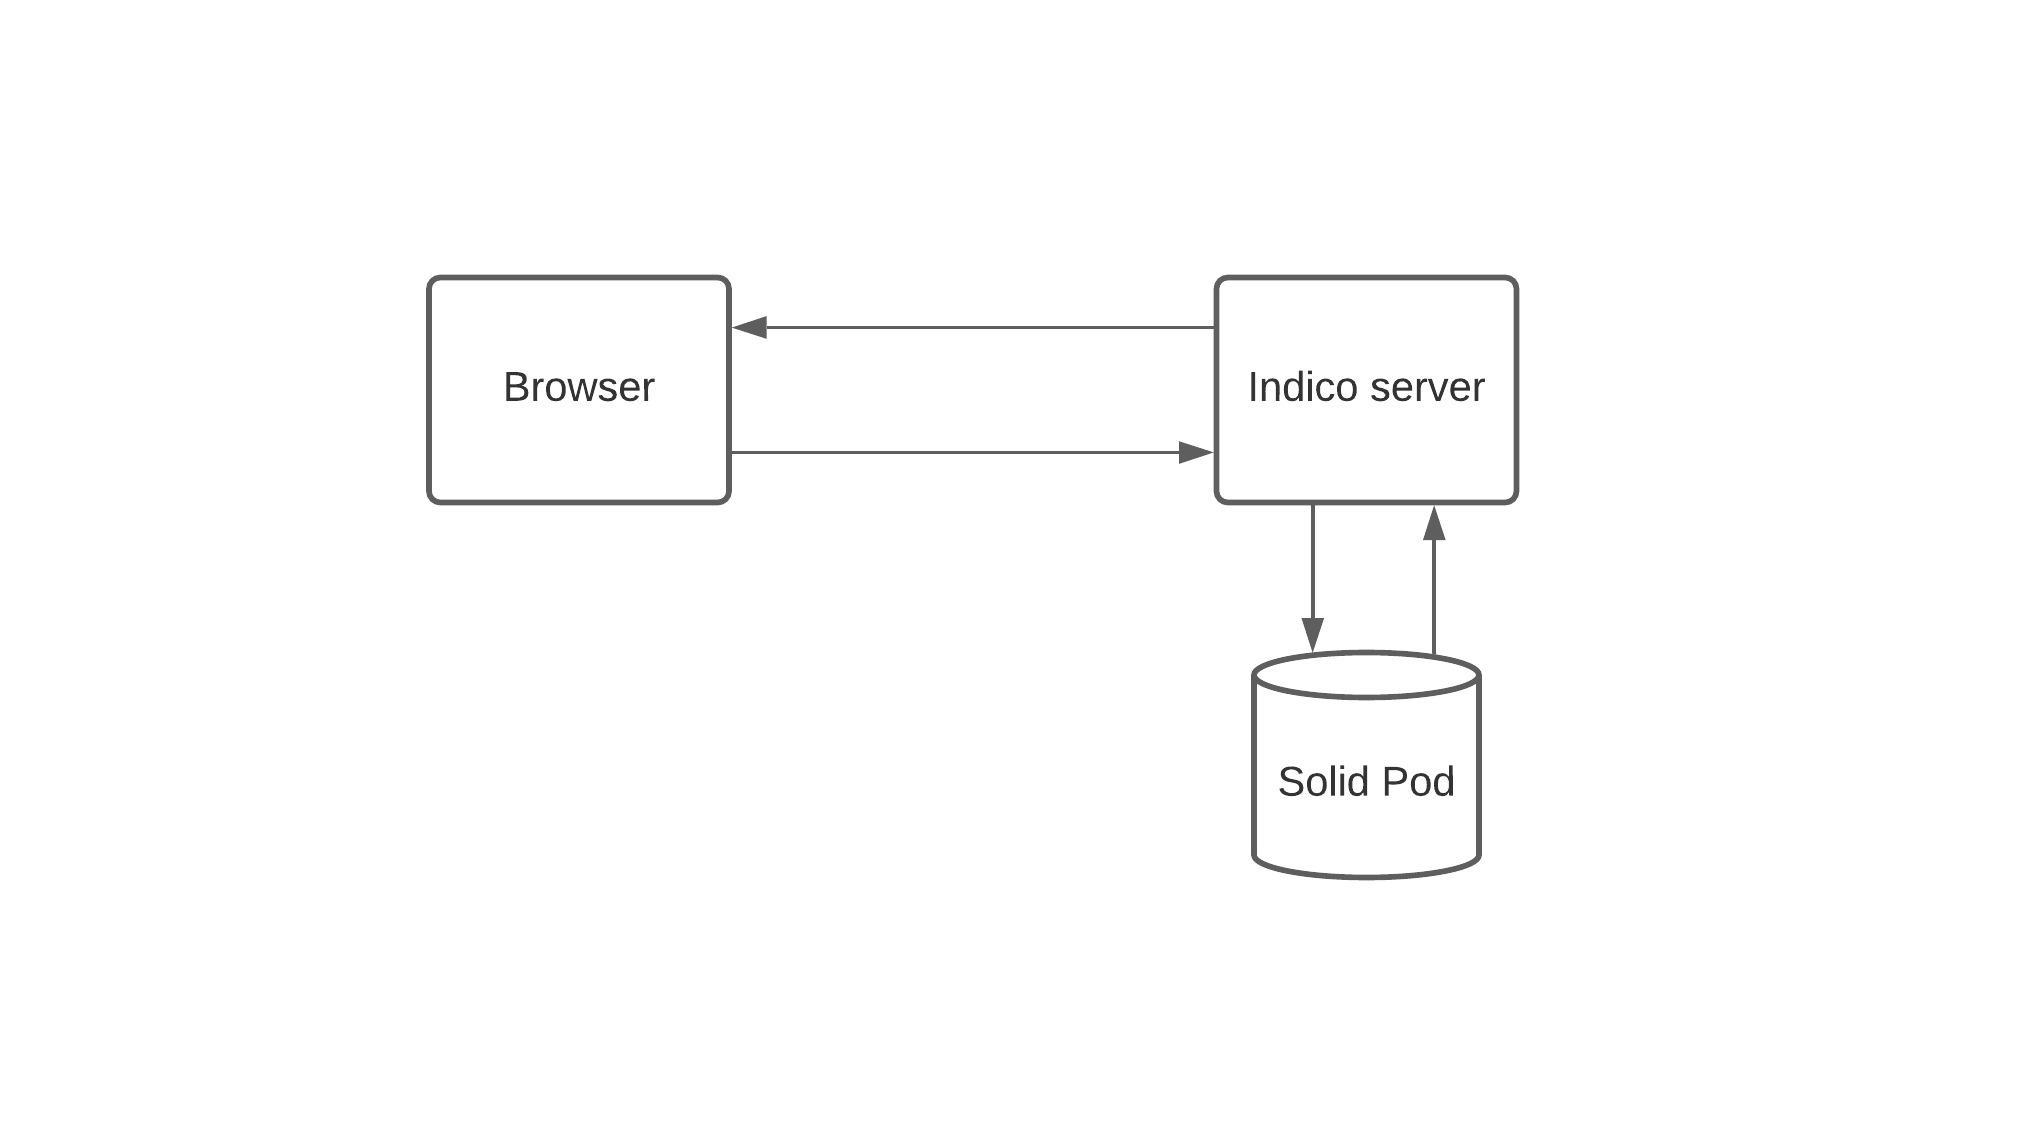
\includegraphics[width=0.8\textwidth]{prototype/graphs/poc-infrastructure-backend.jpeg}
    \caption{Communication flow for a module developed on the server.}
    \label{fig:poc-infrastructure-backend}
\end{figure}
\vspace{0.5cm}
\paragraph{Comparison of the Different Approaches}\mbox{}\\

Benefits from developing the module for the client:

\begin{itemize}
    \item Necessary libraries exist (Major release for all basic Solid flows exist)
    \item Community support
    \item Programming effort for an \gls{mvp} lowest
    \item Documentation on developing Solid apps in \gls{js} exist
\end{itemize}

\begin{table}[h!]
    \centering
    \begin{tabular}{| l | p{11cm} |} 
    \hline
     Library & Description \\
     \hline
      solid-client & A client library for accessing data stored in Solid Pods.  \\
      \hline
      solid-client-authn & A set of libraries for authenticating to Solid identity servers:solid-client-authn-browser for use in a browser.solid-client-authn-node for use in Node.js.  \\
      \hline
      vocab-common-rdf & A library providing convenience objects for many RDF-related identifiers, such as the Person and familyName identifiers from the Schema.org vocabulary from Google, Microsoft and Yahoo!  \\
      \hline
      vocab-solid-common & A library providing convenience objects for many Solid-related identifiers.  \\
      \hline
      vocab-inrupt-common & A library providing convenience objects for Inrupt-related identifiers.  \\
      \hline
    \end{tabular}
    \vspace{0.75cm}
    \caption{Existing solutions to problems for a server approach.}
    \label{table:4}
\end{table}
\vspace{0.5cm}
\paragraph{Storage Location of the Comments}\mbox{}\\

TODO: 

\vspace{0.5cm}
\paragraph{Single Versus Multiple Resource(s) for Comments}\mbox{}\\
Storing the comments in \gls{rdf} can be done in two ways: storing it in one file as a graph with a list of comments, or creating a file for every comment.

\begin{figure}
    \centering
    \begin{subfigure}{.5\textwidth}
      \centering
      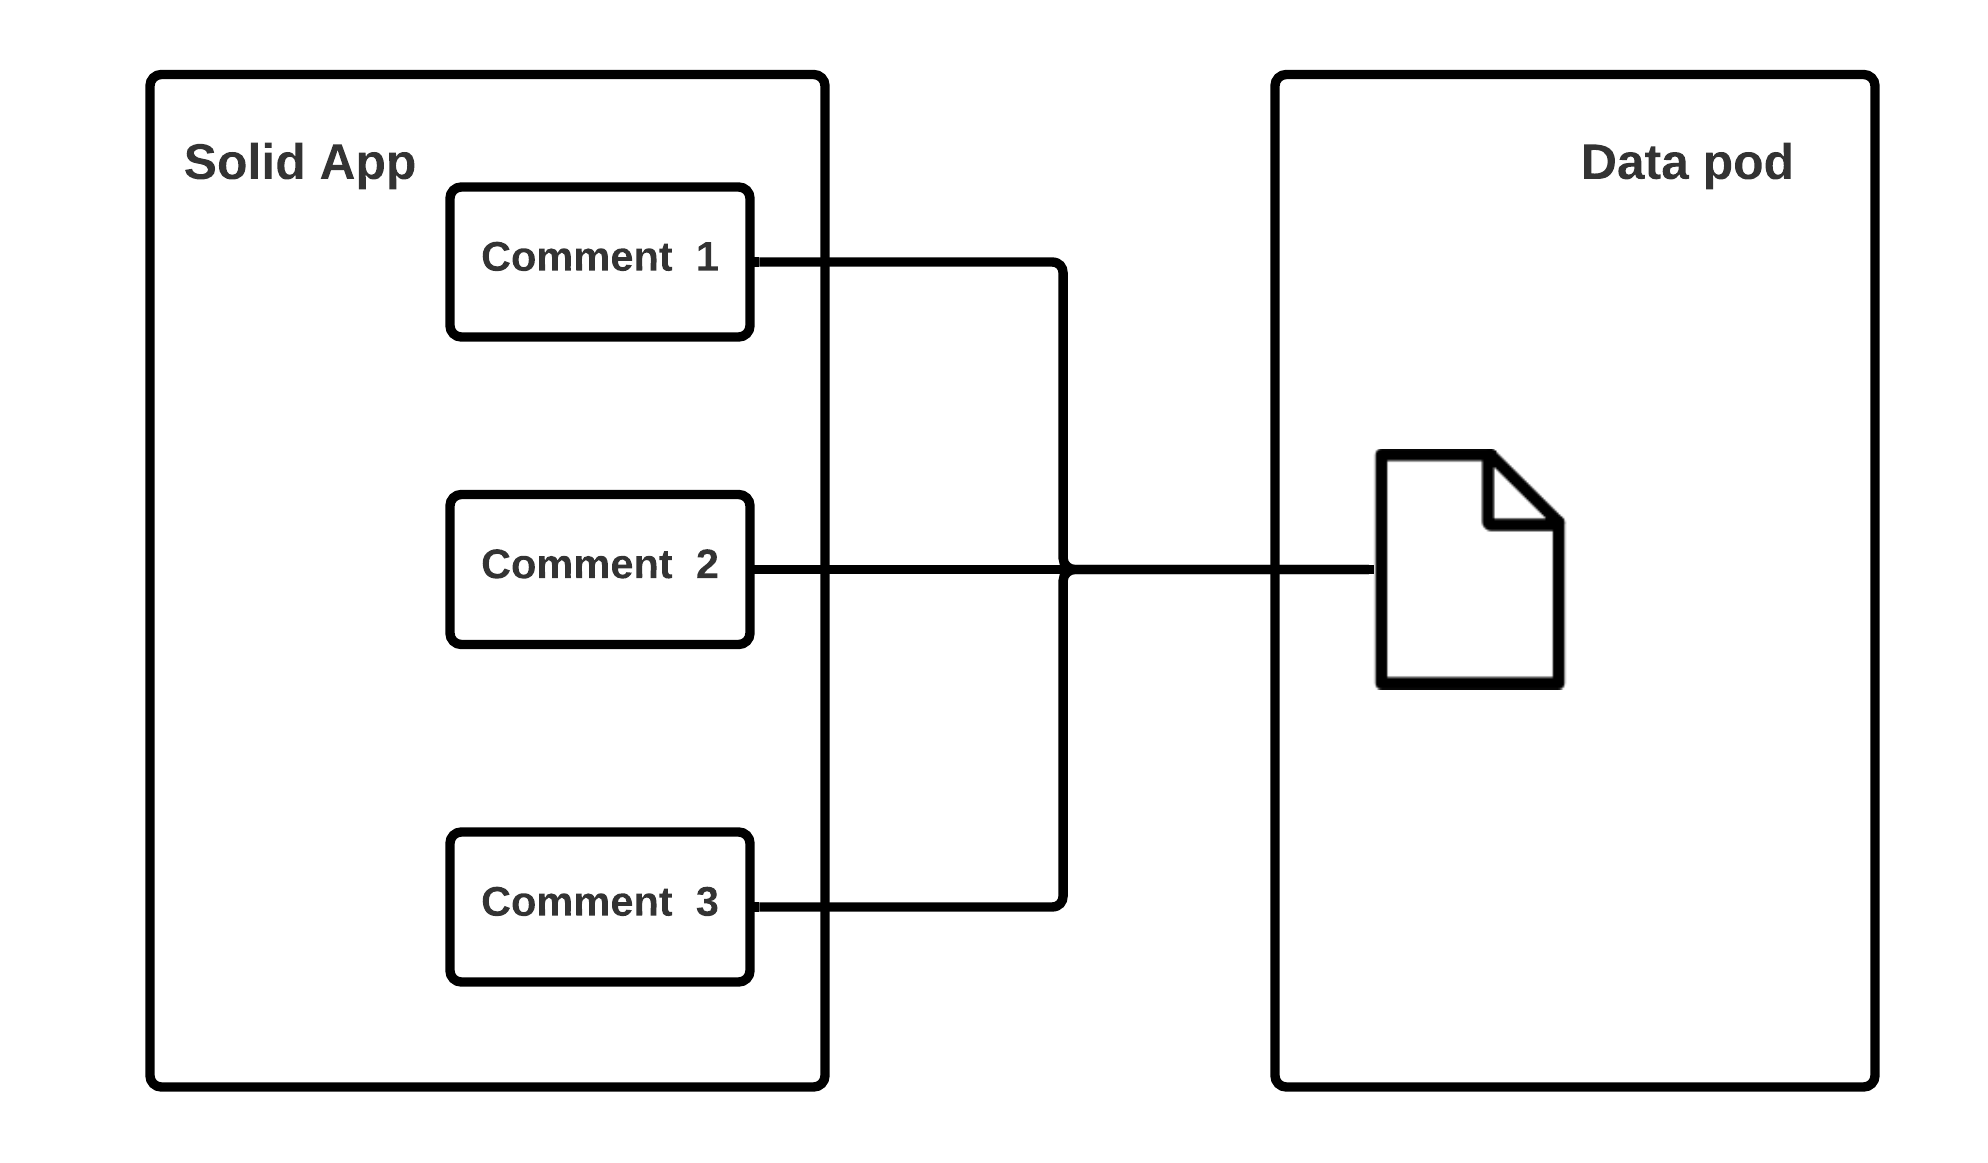
\includegraphics[width=0.7\textwidth]{prototype/graphs/poc-comment-single-resource-comments.png}
      \caption{TODO: caption}
      \label{fig:ppc-comment-single-resource-comments}
    \end{subfigure}%
    \begin{subfigure}{.5\textwidth}
      \centering
      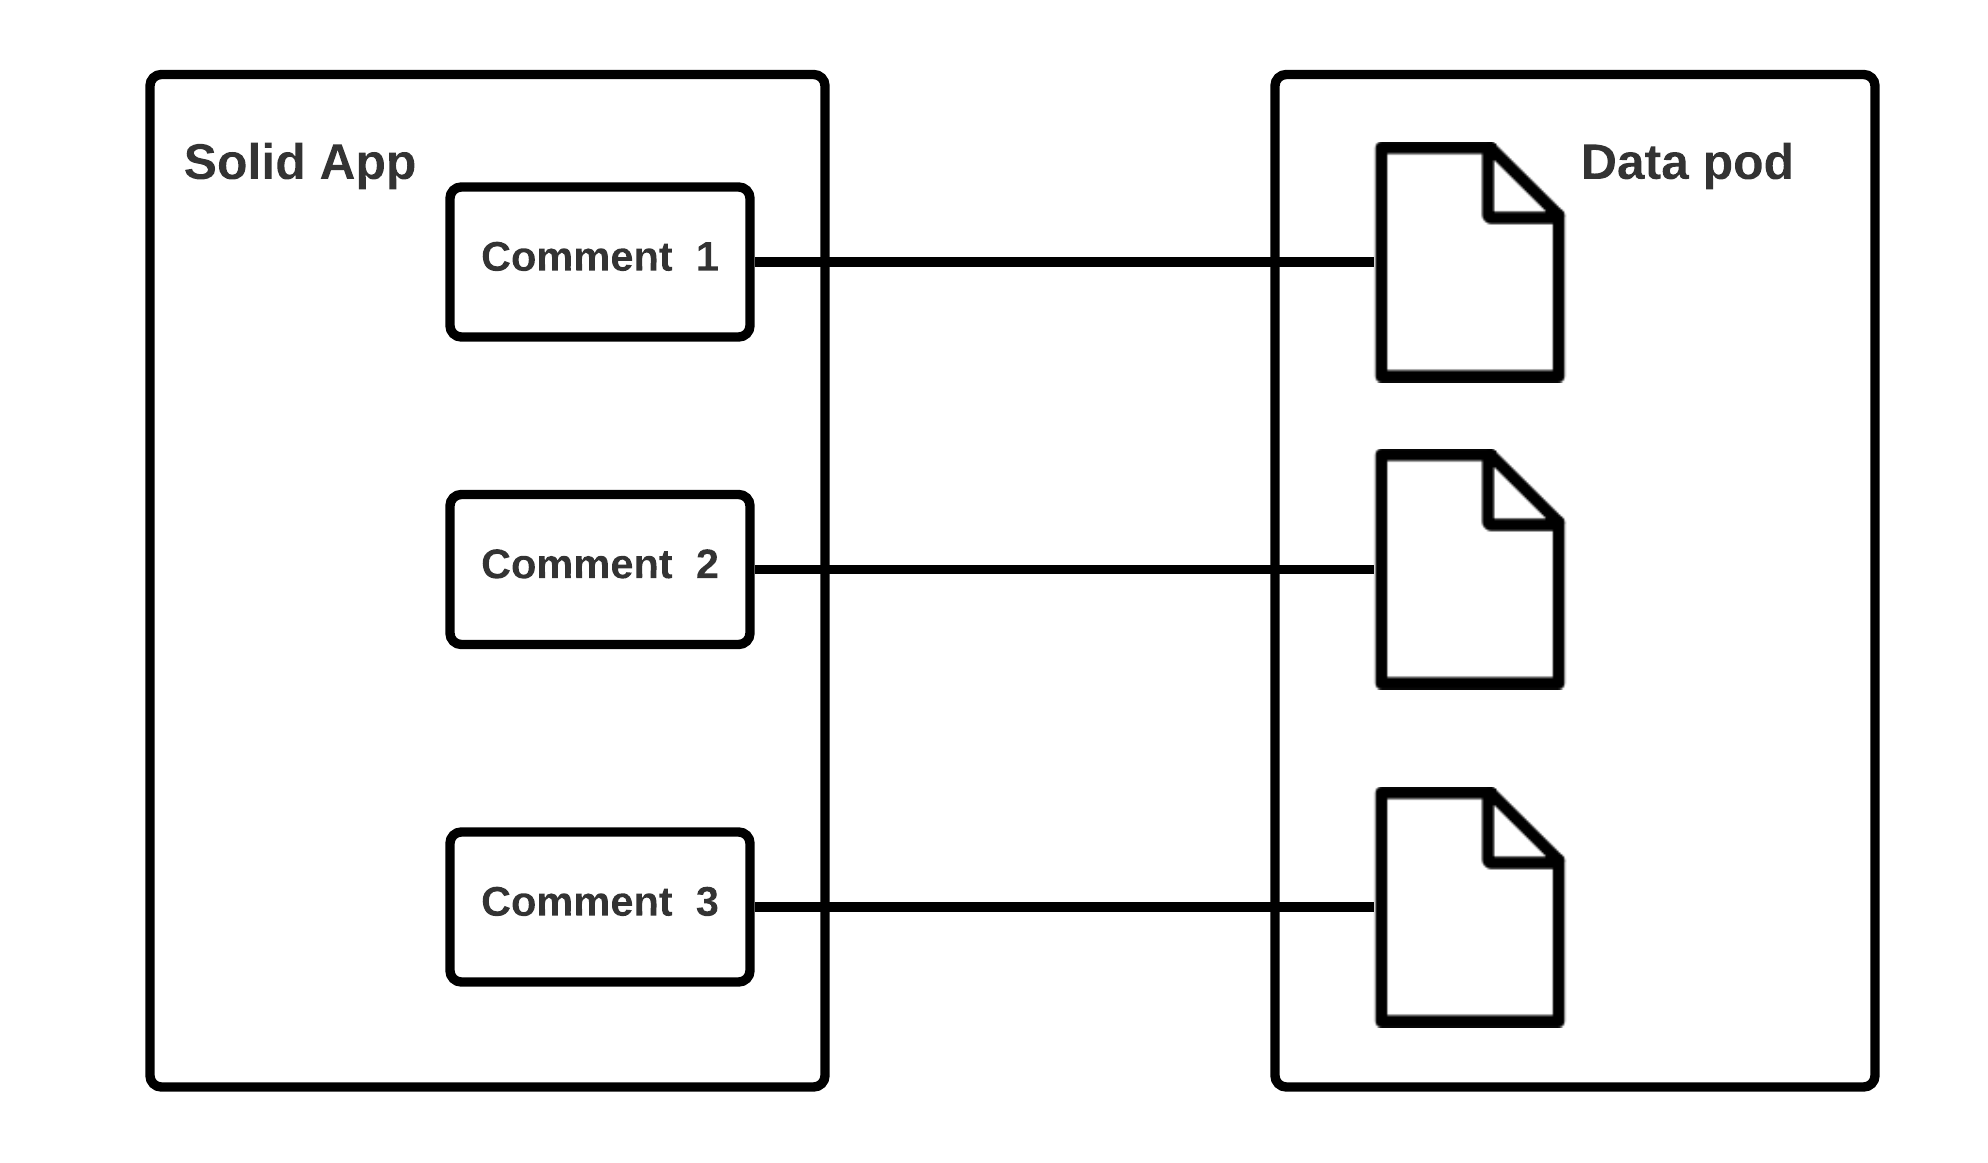
\includegraphics[width=0.7\textwidth]{prototype/graphs/poc-comment-multiple-resources-comments.png}
      \caption{TODO: caption}
      \label{fig:poc-comment-multiple-resources-comments}
    \end{subfigure}
    \caption{TODO: two approaches}
    \label{fig:test}
\end{figure}

When fetching the container with all the comment resources the request returns a Turtle file describing the container, but not the actual content of the contained resources. The misconception of receiving the content as well was thought to be a problem, as it was assumed an initial request to the container reading its child resources had to be made, and then for each resource a request needed to be built to retrieve the resource. This overhead was later disproved as the application where this module is embedded maintains the list of resources to be fetched. Therefore, no manual building of requests to those resources had to be done. The next paragraph also lays out how this design would not work with the protection of the resources.

\vspace{0.5cm}
\paragraph{Protection on Resource}\label{protection-on-resource}\mbox{}\\

Every container and resource in Solid is protected with \gls{wac}, which determines if specific agents, groups, or the world can have read, write, append, or control access. These control access modes are defined in \gls{acl} files. The Solid \gls{acl} inheritance algorithm looks for an \gls{acl} file attached to a specific resource, if it cannot find one it goes recursively up the file hierarchy and looks for \glspl{acl} on the containers.
Indico allows two general types of protection \textit{private} and \textit{public} on its events. Public means open to everyone, no Indico account or any type of authorization is needed to see the event. Whereas private can be as fine-grained as only to specific agents or groups. A comment module is only valuable if the comments can be read by anyone and be written by authorized users.

In order for visitors of a private or public event in Indico to be able to see the comment, the comment’s \gls{acl} needs to allow the public to read the resource. This can be achieved by using the \textit{public} container, which comes with public-read by default on the \gls{nss} or by creating a new container and setting the \gls{acl} with:

\begin{lstlisting}[language=Other,columns=fullflexible, caption={TODO: Label caption}, label={lst:1}]
@prefix acl: <http://www.w3.org/ns/auth/acl#>.
@prefix foaf: <http://xmlns.com/foaf/0.1/>.

# ... Definition for owner

<#example-container-name>
    a acl:Authorization;
    acl:agentClass foaf:Agent;
    acl:accessTo <./>;
    acl:mode acl:Read.
\end{lstlisting}

Every resource in this container is by definition readable by the public -- if not otherwise stated in a more detailed resource \gls{acl}. The above definition even allows the reading of the container’s content, meaning a request to the container would yield a list of resources in the container. This becomes unpleasant if the Indico event is private and the comments for this Indico event should not be read by the world, which is entirely possible when browsing to the location of a specific data pod and then looking into the public container.

To prevent a random agent to see the contents of a container, the container can be set to private, with the container’s resources still be public. This would allow everyone provided they have the \gls{url} to browse to the public resource and read it, but not look into the resource’s parent container. To achieve this behavior with \gls{acl}, the container needs to just define its owner and no specific rules for the public, as \gls{wac} comes with a default private access control. Each child resource needs to define an \gls{acl} now, allowing public read.
The container’s \gls{acl} would look like the following with just an owner defined:

\begin{lstlisting}[language=Other,columns=fullflexible, caption={TODO: Label caption}, label={lst:2}]
@prefix acl: <http://www.w3.org/ns/auth/acl#>.

<#owner>
    a acl:Authorization;
    acl:agent <https://janschill.net/profile/card#me>;
    acl:accessTo <./>;
    acl:default <./>;
    acl:mode acl:Read, acl:Write, acl:Control.
\end{lstlisting}

A child resource would allow public read with:

\begin{lstlisting}[language=Other,columns=fullflexible, caption={TODO: Label caption}, label={lst:3}]
@prefix : <#>.
@prefix acl: <http://www.w3.org/ns/auth/acl#>.
@prefix foaf: <http://xmlns.com/foaf/0.1/>.

# ... Definition for owner

:Read
    a acl:Authorization;
    acl:accessTo <test.txt>;
    acl:agentClass foaf:Agent;
    acl:mode n0:Read.
\end{lstlisting}

Another approach and the one implemented after iterating through the previous ones is to have the container’s \gls{acl} resource define a default access mode for its child resources. This way one \gls{acl} only needs to be created on the container and all resources have proper access modes for public read and are not listed publicly in the container’s description.

\begin{lstlisting}[language=Other,columns=fullflexible, caption={TODO: Label caption}, label={lst:4}]
@prefix acl: <http://www.w3.org/ns/auth/acl#>.
@prefix foaf: <http://xmlns.com/foaf/0.1/>.
@prefix target: <./>.

:ReadDefault
    a acl:Authorization;
    acl:default target:;
    acl:agentClass foaf:Agent;
    acl:mode acl:Read.
\end{lstlisting}
\vspace{0.5cm}
\paragraph{Preventing Unwanted Discovery for Resources}\mbox{}\\

With the resources having proper access modes but being publicly readable a simple naming convention of taking the \gls{iso} 8601 string and using it as a filename for the resources created on the data pod does not suffice -- even though it is a good strategy when looking for a reliable naming convention to prevent duplication. Considering performance improvements such as pagination for future iterations of the module, which would require some sort of iterative indication, a combination of randomness, but also an order indicator it was settled for using \gls{uuid} plus the \gls{iso} 8601 string to form a filename.

Other ideas included hashing a random string with the timestamp to generate non-guessable filenames. The filename would need to use the same hash function to decipher the filename to figure out when the comment was generated. \gls{uuid} is a reliable and easy-to-use system to generate \textit{truly} globally unique strings. 
\vspace{0.5cm}
\paragraph{Modification of Resource From Data Pod}\mbox{}\\

When the users are in control of their data it means they can revoke access any time, or even change their data to their liking. This means when the comment is initially created through Indico and the commenting system's user interface it does not mean this comment needs to remain as is. Even if the interface of the system does not allow modification, a modification can still happen at the source of the storage of the comment.

Regular comment modules usually allow modifications of a submitted text throughout their existence. Twitter is an example where modifications are not allowed after posting \cite{twitter-edit}. 

When this aspect was discovered it was decided to allow this sort of behavior, as it seems to be a natural in this context to be able to edit one's own comments.

\vspace{0.5cm}
\paragraph{Mitigation of Spam}\mbox{}\\

Enabling user input in form of a comment module without application authentication is a gateway to spam. Even though authentication with a Solid \gls{idp} is necessary, it does not hinder a malicious actor to create a multitude of Solid accounts and spam into the application. In the first iteration of the module, only Solid authentication was integrated into the module and would therefore allow anyone with a Solid account to post comments and thus also spam the Indico event theoretically. In a second iteration of the module, another authentication layer was added to mitigate spam from outside Indico. For \gls{cern}’s use-case, an authenticated Indico session was enough. This adds an extra step to the comment process and it is ensured only registered Indico users can comment.
\vspace{0.5cm}
\paragraph{Giving Application Full Control of Data Pod}\mbox{}\\

To create or change programmatically \glspl{acl} requires \textit{control} access to the container. By default \gls{nss} asks for the permissions when authenticating for the first time in the \gls{solidoidc} flow between the \textit{solid-comment} module and Solid \gls{idp}. The permissions granted to the application are on the root container of the data pod. Meaning, giving an application control access allows the application to read, write, change \glspl{acl} on the entire data pod. This is obviously troubling, as a simple application as a commenting module needs to have control access to set the needed \glspl{acl} for the containers and resources it creates.

The current implementation has not a built-in solution, but one way of solving it is the use of an application launcher, which is an application itself with full control access and then limits the access controls of the \textit{solid-comment} module by creating a dedicated container for it and setting the needed \gls{acl} for this specific container only.

\subsubsection{Integration with Indico}\mbox{}\\

The need for integration with Indico is twofold: serving the module to the client and being the provider to the list of references to the comments that have been posted on a specific event.
\vspace{0.5cm}
\paragraph{Storing Reference to Comments in Indico}\mbox{}\\
Indico operates using the relational database PostgreSQL \cite{postgresql}. When a comment gets posted and stored on an external data pod a reference to the location of the comment needs to be kept in order for Indico to pull the comment and render it in its frontend. Several possibilities are imaginable. 


\vspace{0.5cm}
\paragraph{Enforce Authenticated Session For Posting Comments}\mbox{}\\

\subsubsection{Evaluation}\mbox{}\\

This section focuses on evaluating the module. This shall be done by iterating through the module's requirements from the stakeholders and how the architecture lives up to those expectations. The evaluation is done with the help of the \gls{asqa} framework to ensure continuous quality assessment and prioritizing with a lightweight technique \cite{asqa-paper}.
\gls{asqa} contains seven process steps as shown in figure \ref{fig:asqa-process-steps}.

\begin{figure}
    \centering
    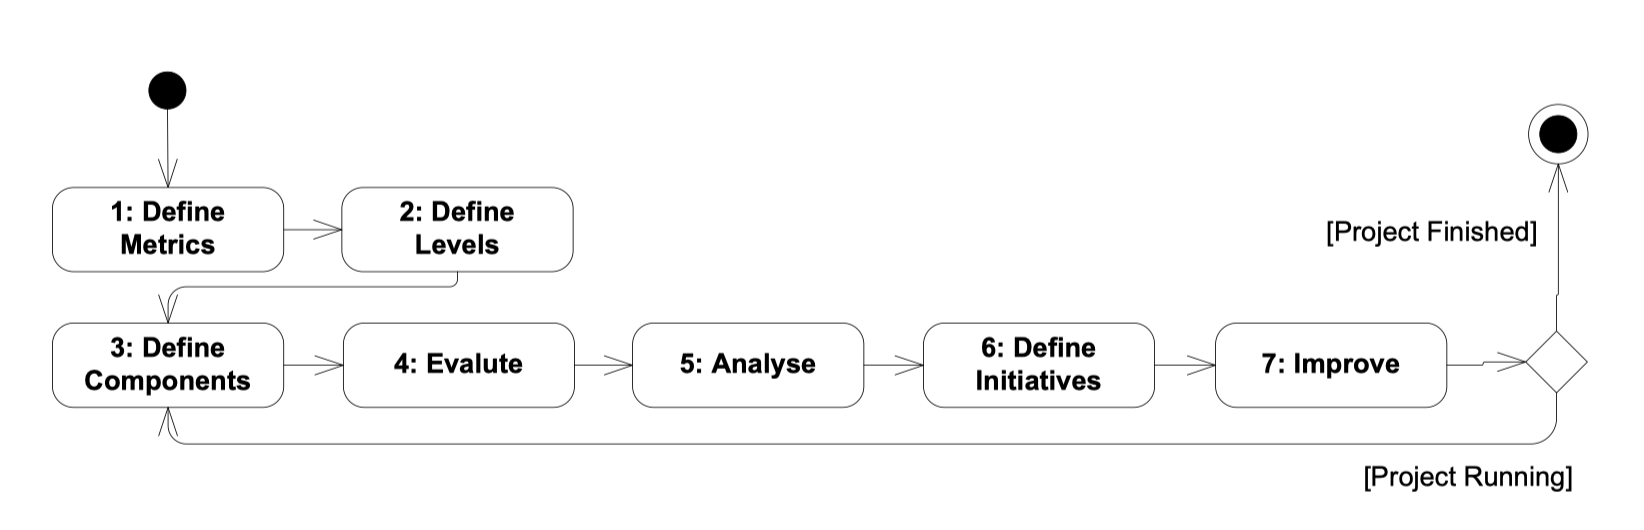
\includegraphics[width=0.7\textwidth]{thesis/latex/assets/asqa-process-steps.png}
    \caption{aSQA Process Steps from \cite{asqa-paper}}
    \label{fig:asqa-process-steps}
\end{figure}
\vspace{0.5cm}
\paragraph{Metrics}\mbox{}\\

Scenario-based metrics were chosen to measure the quality attributes. The different scenarios are predicted to be the most common actions on the system and thus will stress the system and its architecture the most based on the quality attributes.

The iterate over the previously picked quality attributes:

% \vspace{-12mm}

\begin{enumerate}
    \item Security
    \item Performance
    \item Usability
\end{enumerate}

% \vspace{-12mm}

Possible scenarios are centered around data not being available or altered or scenarios of malicious behavior from an adversary by injecting code to misuse the system in unintended ways:

% \vspace{-12mm}

\begin{enumerate}
    \item A user who has commented deletes their comment in their data pod
    \item A user who has commented deletes their data pod
    \item An adversary uses a script to generate a large number of comments
    \item An adversary creates a comment with a \gls{xss} attack
    \item An adversary serves different resources based on client \gls{ip} address
\end{enumerate}

% \vspace{-12mm}
\vspace{0.5cm}
\paragraph{Levels}\mbox{}\\

TODO:
\vspace{0.5cm}
\paragraph{Components}\mbox{}\\

TODO:
\vspace{0.5cm}
\paragraph{Scenarios}\mbox{}\\

TODO:
\subsubsection{Analysis}\mbox{}\\

TODO:
\vspace{0.5cm}
\paragraph{Performance}\mbox{}\\

The chosen technique of storing the comments is not as efficient as it could be. Every comment is stored as a self-contained Turtle file on the author's comment with Indico holding the \gls{uri} to be able to fetch it on demand. As soon as the client is loading the module with the comments the client will have to make $n$ requests, $n$ being the number of comments.

The first improvement to this approach could be pagination. Pagination limits the number of initially loaded comments to a defined amount. This can be achieved by utilizing the date and time from the file name of the comment. Only the most recent $n$ comments by time will have to be fetched. When the user clicks on a load more comments button, $n$ more comments will be loaded.
In the same area of improvement, the ways the comments are rendered can also be improved. The comments as of now will all be fetched and only when all requests are done it will be rendered in the \gls{dom}. If the comments are \textit{separated} from each other and a comment is rendered as soon as it successfully fetched, it would speed up the time until a user could start seeing comments.

Second improvement could be a grouping of comments by author. This way the number of request would now be bound to the number of authors. In the worst case, where all comments are from different authors, it would not bring any improvement over the initial architecture. The design for this would be to change the storage from the multi-file approach to a single-file approach. On the data pod one file would exist holding all comments from one author for one event. This file can be fetched with one request containing multiple comments.
% Another way of achieving this is to use a more efficient asset providing web protocol, such as \gls{http}/2. \gls{http}/2 uses a clever technique to 

Another enhancement can be attained by caching. In its current design the comments are freshly fetched on each page load. Server-side \gls{http} caching is out of control for the clients, and completely relies on the Server implementations to do so. By Solid specification \gls{http} caching is prescribed, but not vital \cite{solid-protocol}, which means it \textit{should} implement it, but does not have to. Regardless, the improvement would not be in the number of round trips the client has to complete, but rather in the time for the server to calculate the response it sends out \cite{http-caching}. A real improvement on consecutive page visits are won by client-side \gls{http} caching. Upon successive visits to a cached website a previously fetched and in the browser's local storage stored copy of the response would be served \cite{http-caching}. The result would be immediately loaded, but might not serve the latest and up-to-date asset from the server. The \textit{freshness} of the response is controlled using the \texttt{Cache-Control} header in either the request or response of the \gls{http} exchange between client and server \cite{http-caching}. 

More performance solutions shall be looked at with the other upcoming areas in this analysis section.
\vspace{0.5cm}
\paragraph{Modification of Resources}\mbox{}\\

In the case of comments being the resources that are being shared between data pod and application it has been established a modification from outside the application is acceptable behavior. For a resource where a modification should be monitored or even forbidden. A few paths are conceivable.

Storing the comments on the author's data pod could be given up and instead be done by a trusted entity, e.g. the application embedding the comment module. It would result in \gls{cern} hosting one data pod for their Indico instance. Each event would create a container in this data pod with \textit{append} access mode for the public. \textit{append} allows an agent to add new resources to a container, but not modify or delete any \cite{solid-protocol}. Through this access mode a user can post comments freely, but cannot modify them at a later stage, as the data is now in Indico's data pod and the user is lacking the access control to edit existing resources. Having one data pod responsible for all comments also improves the performance by reducing the number of \gls{http} requests needed. Whereas before the requests where either bound to the number of authors or even by the number of comments, it is now only a single request to the event's container on the Indico data pod, to fetch a single file with all comments written in. A drawback to this approach is the comments are again stored centralized in one storage, though because it is using a Solid server instead of a web server with unstructured data storage, the data is now structured and thus interoperable through \textit{Linked Data}. Besides storing it in Indico's data pod, a copy of the comment could be stored in the author's data pod. The author acquires a version of the comment and Indico holds the \gls{ssot}.

One more option to control the modification on resources while not giving up on decentralized storage in the author's pods is to use versioning on the comments. Indico would when a user creates and submits a comment store a hashed value of the comment's content. When then serving the comments from the external data pods to visiting clients the received comments would be hashed and compared to the in Indico stored hash value. It is important to associate the comment's \gls{url} with the hash to be able to make a proper comparison on the correct resources.

An important aspect of allowing the update of existing resources is to have an indication in the user interface notifying readers about a changed text. A simple \textit{edited}-hint would suffice. When a user is browsing the comments and follows a conversation, which is met with an abrupt disruption of flow in the conversation an updated comments could be the result and indication would help to identify such situation.  To detect a change in the comment's content the same hashing functionality can be used as described before.



* EventProxy is not scalable, when comments are sent at the same time could be overwritten
* log IP and blog on spam
* extra layer api to cache comments, performance and security against IP logging
* one pod sends different content to users depending on their location
* Performance of petabytes?
* trustworthiness of the data